% ****** Start of file aipsamp.tex ******
%
%   This file is part of the AIP files in the AIP distribution for REVTeX 4.
%   Version 4.1 of REVTeX, October 2009
%
%   Copyright (c) 2009 American Institute of Physics.
%
%   See the AIP README file for restrictions and more information.
%
% TeX'ing this file requires that you have AMS-LaTeX 2.0 installed
% as well as the rest of the prerequisites for REVTeX 4.1
%
% It also requires running BibTeX. The commands are as follows:
%
%  1)  latex  aipsamp
%  2)  bibtex aipsamp
%  3)  latex  aipsamp
%  4)  latex  aipsamp
%
% Use this file as a source of example code for your aip document.
% Use the file aiptemplate.tex as a template for your document.
\documentclass[%
 aip,
 % apl,
% jmp,%
% bmf,%
% sd,%
% rsi,%
 amsmath,amssymb,
% preprint,%
 reprint,%
% author-year,%
% author-numerical,%
 floatfix,%
]{revtex4-1}

\usepackage[utf8]{inputenc}
\usepackage{tikz}
\usepackage{graphicx}% Include figure files
\usepackage{dcolumn}% Align table columns on decimal point
\usepackage[T1]{fontenc}
\usepackage{bm}% bold math
\usepackage{mathptmx}
%\usepackage[mathlines]{lineno}% Enable numbering of text and display math
%\linenumbers\relax % Commence numbering lines
\usetikzlibrary{arrows,decorations.markings,decorations.pathmorphing, patterns,shapes}

\begin{document}

\preprint{AIP/123-QED}

\title[]{The Double Pendulum:\\Creating a Better Baseball Bat}
%\thanks{Footnote to title of article.}

\author{Jared Baur}
%\altaffiliation[Also at ]{Physics Department, Occidental College.}%Lines break automatically or can be forced with \\

\date{\today}% It is always \today, today,
             %  but any date may be explicitly specified

\begin{abstract}
	abstract goes here
\end{abstract}

\maketitle

\onecolumngrid

\section{\label{sec:level1}Introduction}
The double pendulum is a classic example of chaotic motion. The trajectories of various trials will show that the motion of a double pendulum is highly unpredictable. The chaos in a classic double pendulum is described by Equation 1. The exponent $\lambda$ is a positive constant, $\Delta x$ is the trajectory of the bottom arm of the pendulum, and $t$ is time. For small times $t$, the trajectories are relatively the same, however for increasing times, the trajectories exponentially increase in distance from trial to trial.
\begin{equation}
	\Delta x(t) \sim \Delta x(t_0) e^{\lambda t}
\end{equation}

\begin{figure}
	\centering
	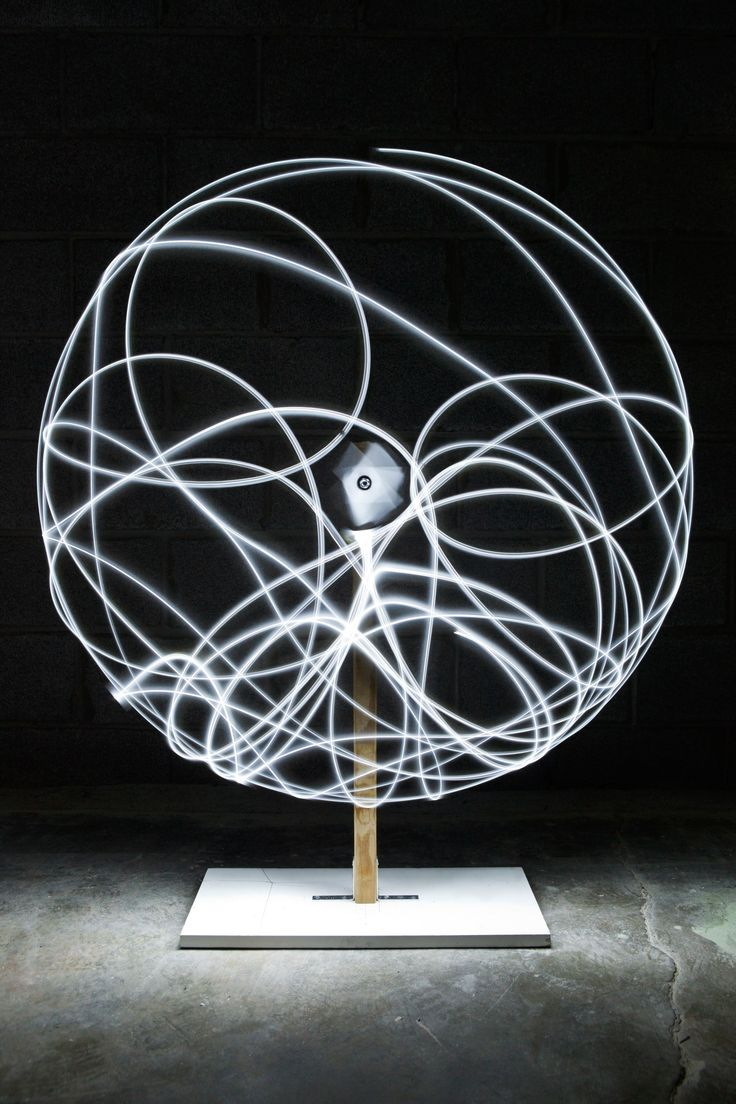
\includegraphics[scale=0.25]{lights.jpg}
	\caption{Chaos in a double pendulum. This figure depicts the trajectory of the end of the bottom arm in the double pendulum. The light is traced along the route of the bottom arm. As seen, there is no evident pattern in the bottom arm's trajectory.}
\end{figure}

The double pendulum is used in real life situations such as *to-do:name situations*. The swinging motion in sports is also a common instance of a double pendulum. For this paper, the double pendulum will be compared to a baseball swing. *to-do: explain baseball swing*.

-----

Since the swing of a baseball bat only occurs once (does not swing back and forth and time $t$ is relatively low), this motion translates to the first half cycle of a double pendulum swing. Thus, the chaotic motion prevalent in classic double pendulums will not be applicable for the purpose of the baseball swing.

The double pendulum motion can be compared to the motion of a swing of a baseball bat, golf club, tennis racquet, or any other "swinging" motion that occurs with a striking implement. The focus of this paper will be on the swinging of a baseball bat, which will be our striking implement. The goal of this paper will be to quantitatively describe the double pendulum in the context of a baseball swing and determine whether all of the energy in the striking implement can be transferred to the ball on impact.

-----

\section{\label{sec:level2}Equations of Motion}


		\begin{equation}
			L_1 \sin{\theta} + h_2 \sin{\phi} - L_1 \cos{\theta} - h_2 \cos{\phi}
		\end{equation}

		\begin{equation}
			V_x = \frac{dx}{dt} = -L_1 \omega_1 \cos{\theta} - h_2 \omega_2 \cos{\phi}
		\end{equation}
		\begin{equation}
			V_y = \frac{dy}{dt} = -L_1 \omega_1 \sin{\theta} - h_2 \omega_2 \sin{\phi}
		\end{equation}


		\begin{equation}
			\begin{aligned}
				F_x & = M_2 \frac{d V_x}{dt} \\
				    & = -M_2 \bigg [ L_1 \cos{\theta} \frac{d \omega_1}{dt} + L_1 \omega_1^2 \sin{\theta} + h_2 \cos{\phi} \frac{d \omega_2}{dt} + h_2 \omega_2^2 \sin{\phi} \bigg ]
			\end{aligned}
		\end{equation}

		\begin{equation}
			\begin{aligned}
				F_y - M_2 g & = M_2 \frac{d V_y}{dt}\\
				 % & = \\
				   & = -M_2 \bigg [ L_1 \sin{\theta} \frac{d \omega_1}{dt} - L_1 \omega_1^2 \cos{\theta} + h_2 \sin{\phi} \frac{d \omega_2}{dt} - h_2 \omega_2^2 \cos{\phi} \bigg ]
			\end{aligned}
		\end{equation}







\section{\label{sec:level3}Experimental Results}

\section{\label{sec:level4}Torque}

\section{\label{sec:level5}Energy Transfer}

\section{\label{sec:level6}Conclusion}

\nocite{*}
\bibliography{main.bib}% Produces the bibliography via BibTeX.

\end{document}
%
% ****** End of file aipsamp.tex ******
